%--------------------
% Packages
% -------------------
\documentclass[11pt,english]{article}
\usepackage{amsfonts}
\usepackage[left=2.5cm,top=2cm,right=2.5cm,bottom=3cm,bindingoffset=0cm]{geometry}
\usepackage{amsmath, amsthm, amssymb}
\usepackage{tikz}
\usetikzlibrary{calc}
\usetikzlibrary{decorations.pathreplacing,calligraphy}
\usepackage{fancyhdr}
%\usepackage{currfile}
\usepackage{nicefrac}
\usepackage{cite}
\usepackage{graphicx}
\usepackage{caption}
\usepackage{longtable}
\usepackage{rotating}
\usepackage{lscape}
\usepackage{booktabs}
\usepackage{float}
\usepackage{placeins}
\usepackage{setspace}
\usepackage[font=itshape]{quoting}
\onehalfspacing
\usepackage{mathrsfs}
\usepackage{tcolorbox}
\usepackage{xcolor}
\usepackage{subcaption}
\usepackage{float}
\usepackage[multiple]{footmisc}
\usepackage[T1]{fontenc}
\usepackage[sc]{mathpazo}
\usepackage{listings}
\usepackage{longtable}
\definecolor{cmured}{RGB}{175,30,45}
\definecolor{macroblue}{RGB}{56,108,176}
\usepackage[format=plain,
            labelfont=bf,
            textfont=]{caption}
\usepackage[colorlinks=true,citecolor=macroblue,linkcolor=macroblue,urlcolor=macroblue]{hyperref}
\usepackage{varioref}
\usepackage{chngcntr}
\usepackage{datetime}

\definecolor{darkgreen}{RGB}{30,175,88}
\definecolor{darkblue}{RGB}{30,118,175}
\definecolor{maroon}{rgb}{0.66,0,0}
\definecolor{darkgreen}{rgb}{0,0.69,0}

%Counters
\newtheorem{theorem}{Theorem}[section] 
\newtheorem{proposition}{Proposition}
\newtheorem{lemma}{Lemma}
\newtheorem{corollary}{Corollary}
\newtheorem{assumption}{Assumption}
\newtheorem{axiom}{Axiom}
\newtheorem{case}{Case}
\newtheorem{claim}{Claim}
\newtheorem{condition}{Condition}
\newtheorem{definition}{Definition}
\newtheorem{example}{Example}
\newtheorem{notation}{Notation}
\newtheorem{remark}{Remark}


\hypersetup{ 	
pdfsubject = {},
pdftitle = {TidyTuesday Week 2},
pdfauthor = {Pranay Gundam},
linkcolor= macroblue
}


\title{\textbf{TidyTuesday Week 2}}
\author{Pranay Gundam}


%-----------------------
% Begin document
%-----------------------
\begin{document}

\maketitle

\tableofcontents

\section{Weekly Summary}


\section{Date: 2025-01-06}
\noindent \textbf{Series ID: PE5T17NE31163A647NCEN} 

\noindent This series is titled Estimate of Related Children Age 5-17 in Families in Poverty for Sherman County, NE and has a frequency of Annual. The units are Persons and the seasonal adjustment is Not Seasonally Adjusted.The observation start date is 1989-01-01 and the observation end date is 2023-01-01.The popularity of this series is 0. \\ 

\noindent \textbf{Series ID: NCOALLSRE1FRMACB} 

\noindent This series is titled Asset Quality Measures, Net Charge-Offs on All Loans and Leases, Secured by Real Estate, Single Family Residential Mortgages, Booked in Domestic Offices, All Commercial Banks and has a frequency of Quarterly. The units are Millions of Dollars and the seasonal adjustment is Not Seasonally Adjusted.The observation start date is 1991-01-01 and the observation end date is 2024-07-01.The popularity of this series is 2. \\ 

\subsection{Regression Tables and Plots}
\begin{center}
\begin{tabular}{lclc}
\toprule
\textbf{Dep. Variable:}                     & value\_fred\_NCOALLSRE1FRMACB & \textbf{  R-squared:         } &     0.009   \\
\textbf{Model:}                             &              OLS              & \textbf{  Adj. R-squared:    } &    -0.027   \\
\textbf{Method:}                            &         Least Squares         & \textbf{  F-statistic:       } &    0.2576   \\
\textbf{Date:}                              &        Mon, 06 Jan 2025       & \textbf{  Prob (F-statistic):} &    0.616    \\
\textbf{Time:}                              &            13:19:18           & \textbf{  Log-Likelihood:    } &   -276.39   \\
\textbf{No. Observations:}                  &                 29            & \textbf{  AIC:               } &     556.8   \\
\textbf{Df Residuals:}                      &                 27            & \textbf{  BIC:               } &     559.5   \\
\textbf{Df Model:}                          &                  1            & \textbf{                     } &             \\
\textbf{Covariance Type:}                   &           nonrobust           & \textbf{                     } &             \\
\bottomrule
\end{tabular}
\begin{tabular}{lcccccc}
                                            & \textbf{coef} & \textbf{std err} & \textbf{t} & \textbf{P$> |$t$|$} & \textbf{[0.025} & \textbf{0.975]}  \\
\midrule
\textbf{const}                              &    -329.7910  &     4436.181     &    -0.074  &         0.941        &    -9432.083    &     8772.501     \\
\textbf{value\_fred\_PE5T17NE31163A647NCEN} &      26.0933  &       51.412     &     0.508  &         0.616        &      -79.396    &      131.583     \\
\bottomrule
\end{tabular}
\begin{tabular}{lclc}
\textbf{Omnibus:}       & 20.243 & \textbf{  Durbin-Watson:     } &    0.266  \\
\textbf{Prob(Omnibus):} &  0.000 & \textbf{  Jarque-Bera (JB):  } &   24.859  \\
\textbf{Skew:}          &  1.891 & \textbf{  Prob(JB):          } & 4.00e-06  \\
\textbf{Kurtosis:}      &  5.504 & \textbf{  Cond. No.          } &     597.  \\
\bottomrule
\end{tabular}
%\caption{OLS Regression Results}
\end{center}

Notes: \newline
 [1] Standard Errors assume that the covariance matrix of the errors is correctly specified.

\begin{figure}
\centering
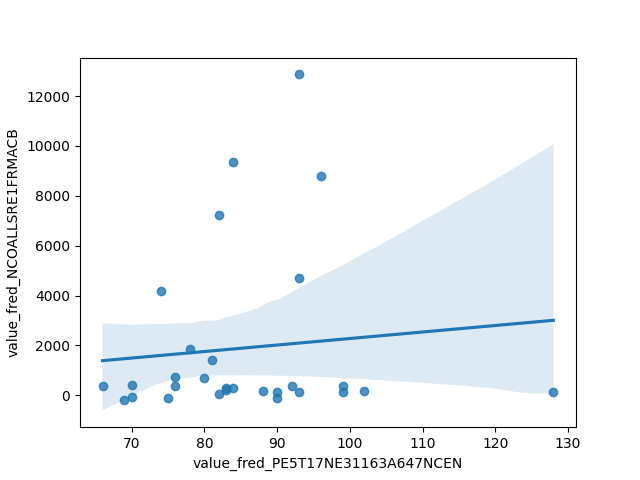
\includegraphics[scale = 0.9]{plots/plot_2025-01-06.png}
\caption{Regression Plot for 2025-01-06}
\end{figure}
\newpage

\section{Date: 2025-01-07}
\noindent \textbf{Series ID: MEANAGINE31A052NCEN} 

\noindent This series is titled Mean Adjusted Gross Income for Nebraska and has a frequency of Annual. The units are Dollars and the seasonal adjustment is Not Seasonally Adjusted.The observation start date is 1989-01-01 and the observation end date is 2022-01-01.The popularity of this series is 1. \\ 

\noindent \textbf{Series ID: RGDPTHJPA630NUPN} 

\noindent This series is titled Purchasing Power Parity Converted GDP Laspeyres per hour worked by employees for Japan and has a frequency of Annual. The units are 2005 International Dollars per Hour and the seasonal adjustment is Not Seasonally Adjusted.The observation start date is 1950-01-01 and the observation end date is 2010-01-01.The popularity of this series is 1. \\ 

\subsection{Regression Tables and Plots}
\begin{center}
\begin{tabular}{lclc}
\toprule
\textbf{Dep. Variable:}                   & value\_fred\_RGDPTHJPA630NUPN & \textbf{  R-squared:         } &     0.960   \\
\textbf{Model:}                           &              OLS              & \textbf{  Adj. R-squared:    } &     0.958   \\
\textbf{Method:}                          &         Least Squares         & \textbf{  F-statistic:       } &     484.1   \\
\textbf{Date:}                            &        Tue, 07 Jan 2025       & \textbf{  Prob (F-statistic):} &  1.73e-15   \\
\textbf{Time:}                            &            12:51:04           & \textbf{  Log-Likelihood:    } &   -24.588   \\
\textbf{No. Observations:}                &                 22            & \textbf{  AIC:               } &     53.18   \\
\textbf{Df Residuals:}                    &                 20            & \textbf{  BIC:               } &     55.36   \\
\textbf{Df Model:}                        &                  1            & \textbf{                     } &             \\
\textbf{Covariance Type:}                 &           nonrobust           & \textbf{                     } &             \\
\bottomrule
\end{tabular}
\begin{tabular}{lcccccc}
                                          & \textbf{coef} & \textbf{std err} & \textbf{t} & \textbf{P$> |$t$|$} & \textbf{[0.025} & \textbf{0.975]}  \\
\midrule
\textbf{const}                            &      14.9471  &        0.755     &    19.796  &         0.000        &       13.372    &       16.522     \\
\textbf{value\_fred\_MEANAGINE31A052NCEN} &       0.0004  &     1.72e-05     &    22.002  &         0.000        &        0.000    &        0.000     \\
\bottomrule
\end{tabular}
\begin{tabular}{lclc}
\textbf{Omnibus:}       &  5.134 & \textbf{  Durbin-Watson:     } &    0.758  \\
\textbf{Prob(Omnibus):} &  0.077 & \textbf{  Jarque-Bera (JB):  } &    3.967  \\
\textbf{Skew:}          & -1.040 & \textbf{  Prob(JB):          } &    0.138  \\
\textbf{Kurtosis:}      &  2.965 & \textbf{  Cond. No.          } & 2.00e+05  \\
\bottomrule
\end{tabular}
%\caption{OLS Regression Results}
\end{center}

Notes: \newline
 [1] Standard Errors assume that the covariance matrix of the errors is correctly specified. \newline
 [2] The condition number is large,  2e+05. This might indicate that there are \newline
 strong multicollinearity or other numerical problems.

\begin{figure}
\centering
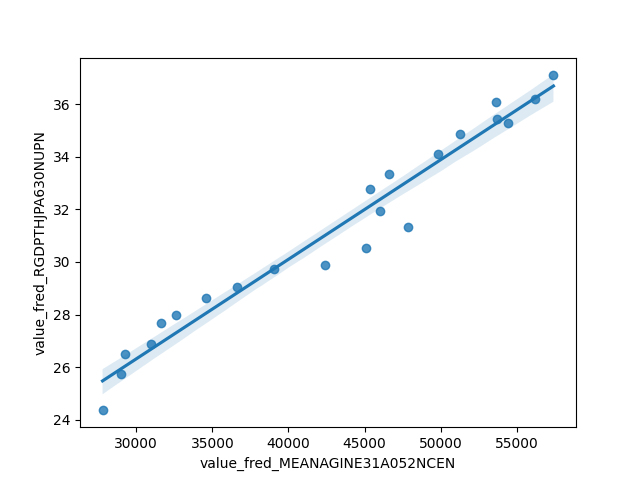
\includegraphics[scale = 0.9]{plots/plot_2025-01-07.png}
\caption{Regression Plot for 2025-01-07}
\end{figure}
\newpage

\section{Date: 2025-01-08}
\noindent \textbf{Series ID: ASTPIRQ027S} 

\noindent This series is titled All Sectors; Taxes on Production and Imports, Receivable (IMA), Transactions and has a frequency of Quarterly. The units are Millions of Dollars and the seasonal adjustment is Seasonally Adjusted Annual Rate.The observation start date is 1946-10-01 and the observation end date is 2024-07-01.The popularity of this series is 1. \\ 

\noindent \textbf{Series ID: O4243MM157SCEN} 

\noindent This series is titled Merchant Wholesalers, Except Manufacturers' Sales Branches and Offices: Nondurable Goods: Apparel, Piece Goods, and Notions Inventories and has a frequency of Monthly, End of Month. The units are Percent and the seasonal adjustment is Seasonally Adjusted.The observation start date is 1992-02-01 and the observation end date is 2024-11-01.The popularity of this series is 1. \\ 

\subsection{Regression Tables and Plots}
\begin{center}
\begin{tabular}{lclc}
\toprule
\textbf{Dep. Variable:}           & value\_fred\_O4243MM157SCEN & \textbf{  R-squared:         } &     0.012   \\
\textbf{Model:}                   &             OLS             & \textbf{  Adj. R-squared:    } &     0.004   \\
\textbf{Method:}                  &        Least Squares        & \textbf{  F-statistic:       } &     1.543   \\
\textbf{Date:}                    &       Wed, 08 Jan 2025      & \textbf{  Prob (F-statistic):} &    0.216    \\
\textbf{Time:}                    &           12:51:13          & \textbf{  Log-Likelihood:    } &   -268.13   \\
\textbf{No. Observations:}        &               130           & \textbf{  AIC:               } &     540.3   \\
\textbf{Df Residuals:}            &               128           & \textbf{  BIC:               } &     546.0   \\
\textbf{Df Model:}                &                 1           & \textbf{                     } &             \\
\textbf{Covariance Type:}         &          nonrobust          & \textbf{                     } &             \\
\bottomrule
\end{tabular}
\begin{tabular}{lcccccc}
                                  & \textbf{coef} & \textbf{std err} & \textbf{t} & \textbf{P$> |$t$|$} & \textbf{[0.025} & \textbf{0.975]}  \\
\midrule
\textbf{const}                    &       0.5960  &        0.467     &     1.277  &         0.204        &       -0.327    &        1.519     \\
\textbf{value\_fred\_ASTPIRQ027S} &   -5.093e-07  &      4.1e-07     &    -1.242  &         0.216        &    -1.32e-06    &     3.02e-07     \\
\bottomrule
\end{tabular}
\begin{tabular}{lclc}
\textbf{Omnibus:}       &  2.213 & \textbf{  Durbin-Watson:     } &    1.410  \\
\textbf{Prob(Omnibus):} &  0.331 & \textbf{  Jarque-Bera (JB):  } &    1.723  \\
\textbf{Skew:}          &  0.252 & \textbf{  Prob(JB):          } &    0.422  \\
\textbf{Kurtosis:}      &  3.253 & \textbf{  Cond. No.          } & 3.16e+06  \\
\bottomrule
\end{tabular}
%\caption{OLS Regression Results}
\end{center}

Notes: \newline
 [1] Standard Errors assume that the covariance matrix of the errors is correctly specified. \newline
 [2] The condition number is large, 3.16e+06. This might indicate that there are \newline
 strong multicollinearity or other numerical problems.

\begin{figure}
\centering
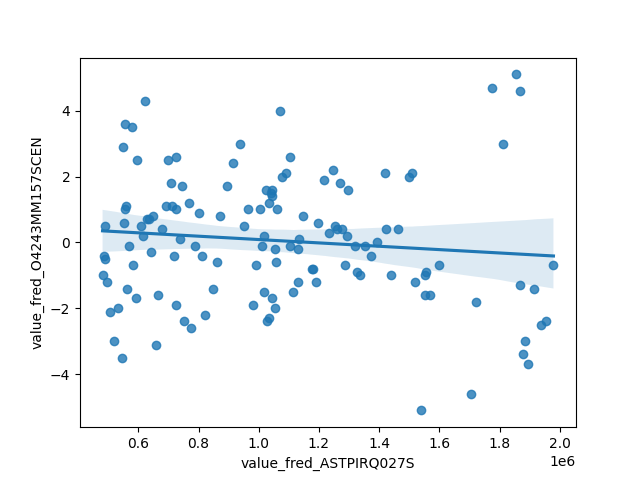
\includegraphics[scale = 0.9]{plots/plot_2025-01-08.png}
\caption{Regression Plot for 2025-01-08}
\end{figure}
\newpage

\section{Date: 2025-01-09}
\noindent \textbf{Series ID: INJPOIPIMEPS} 

\noindent This series is titled Medical Services Expenditures by Disease: Injury and Poisoning Price Index, MEPS Account Basis and has a frequency of Annual. The units are Index 2017=100 and the seasonal adjustment is Not Seasonally Adjusted.The observation start date is 2000-01-01 and the observation end date is 2021-01-01.The popularity of this series is 1. \\ 

\noindent \textbf{Series ID: NA000252Q} 

\noindent This series is titled Gross Domestic Income: Compensation of Employees, Paid and has a frequency of Quarterly. The units are Millions of Dollars and the seasonal adjustment is Not Seasonally Adjusted.The observation start date is 2002-01-01 and the observation end date is 2024-07-01.The popularity of this series is 1. \\ 

\subsection{Regression Tables and Plots}
\begin{center}
\begin{tabular}{lclc}
\toprule
\textbf{Dep. Variable:}            & value\_fred\_NA000252Q & \textbf{  R-squared:         } &     0.867   \\
\textbf{Model:}                    &          OLS           & \textbf{  Adj. R-squared:    } &     0.859   \\
\textbf{Method:}                   &     Least Squares      & \textbf{  F-statistic:       } &     116.9   \\
\textbf{Date:}                     &    Thu, 09 Jan 2025    & \textbf{  Prob (F-statistic):} &  2.66e-09   \\
\textbf{Time:}                     &        11:49:32        & \textbf{  Log-Likelihood:    } &   -269.24   \\
\textbf{No. Observations:}         &             20         & \textbf{  AIC:               } &     542.5   \\
\textbf{Df Residuals:}             &             18         & \textbf{  BIC:               } &     544.5   \\
\textbf{Df Model:}                 &              1         & \textbf{                     } &             \\
\textbf{Covariance Type:}          &       nonrobust        & \textbf{                     } &             \\
\bottomrule
\end{tabular}
\begin{tabular}{lcccccc}
                                   & \textbf{coef} & \textbf{std err} & \textbf{t} & \textbf{P$> |$t$|$} & \textbf{[0.025} & \textbf{0.975]}  \\
\midrule
\textbf{const}                     &    2.208e+05  &     1.89e+05     &     1.166  &         0.259        &    -1.77e+05    &     6.19e+05     \\
\textbf{value\_fred\_INJPOIPIMEPS} &    2.109e+04  &     1950.718     &    10.811  &         0.000        &      1.7e+04    &     2.52e+04     \\
\bottomrule
\end{tabular}
\begin{tabular}{lclc}
\textbf{Omnibus:}       &  0.474 & \textbf{  Durbin-Watson:     } &    0.674  \\
\textbf{Prob(Omnibus):} &  0.789 & \textbf{  Jarque-Bera (JB):  } &    0.211  \\
\textbf{Skew:}          &  0.241 & \textbf{  Prob(JB):          } &    0.900  \\
\textbf{Kurtosis:}      &  2.857 & \textbf{  Cond. No.          } &     459.  \\
\bottomrule
\end{tabular}
%\caption{OLS Regression Results}
\end{center}

Notes: \newline
 [1] Standard Errors assume that the covariance matrix of the errors is correctly specified.

\begin{figure}
\centering
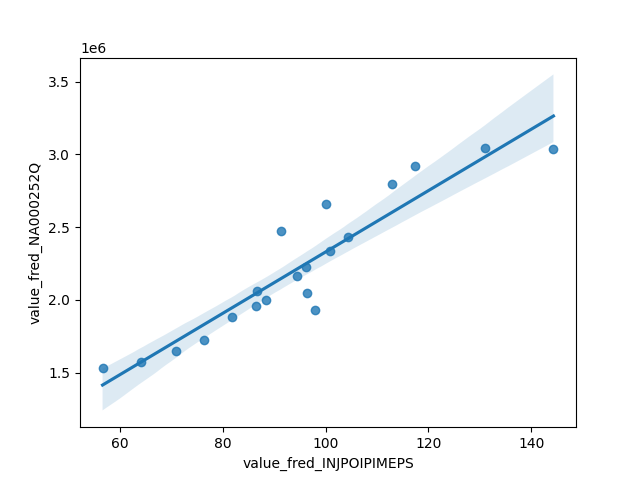
\includegraphics[scale = 0.9]{plots/plot_2025-01-09.png}
\caption{Regression Plot for 2025-01-09}
\end{figure}
\newpage

\section{Date: 2025-01-10}
\noindent \textbf{Series ID: INJPOIPIMEPS} 

\noindent This series is titled Medical Services Expenditures by Disease: Injury and Poisoning Price Index, MEPS Account Basis and has a frequency of Annual. The units are Index 2017=100 and the seasonal adjustment is Not Seasonally Adjusted.The observation start date is 2000-01-01 and the observation end date is 2021-01-01.The popularity of this series is 1. \\ 

\noindent \textbf{Series ID: CMDEBT} 

\noindent This series is titled Households and Nonprofit Organizations; Debt Securities and Loans; Liability, Level and has a frequency of Quarterly, End of Period. The units are Billions of Dollars and the seasonal adjustment is Seasonally Adjusted.The observation start date is 1945-10-01 and the observation end date is 2024-07-01.The popularity of this series is 43. \\ 

\subsection{Regression Tables and Plots}
\begin{center}
\begin{tabular}{lclc}
\toprule
\textbf{Dep. Variable:}            & value\_fred\_CMDEBT & \textbf{  R-squared:         } &     0.855   \\
\textbf{Model:}                    &         OLS         & \textbf{  Adj. R-squared:    } &     0.848   \\
\textbf{Method:}                   &    Least Squares    & \textbf{  F-statistic:       } &     118.3   \\
\textbf{Date:}                     &   Fri, 10 Jan 2025  & \textbf{  Prob (F-statistic):} &  7.54e-10   \\
\textbf{Time:}                     &       08:22:51      & \textbf{  Log-Likelihood:    } &   -184.48   \\
\textbf{No. Observations:}         &            22       & \textbf{  AIC:               } &     373.0   \\
\textbf{Df Residuals:}             &            20       & \textbf{  BIC:               } &     375.1   \\
\textbf{Df Model:}                 &             1       & \textbf{                     } &             \\
\textbf{Covariance Type:}          &      nonrobust      & \textbf{                     } &             \\
\bottomrule
\end{tabular}
\begin{tabular}{lcccccc}
                                   & \textbf{coef} & \textbf{std err} & \textbf{t} & \textbf{P$> |$t$|$} & \textbf{[0.025} & \textbf{0.975]}  \\
\midrule
\textbf{const}                     &    2480.2396  &      980.754     &     2.529  &         0.020        &      434.423    &     4526.056     \\
\textbf{value\_fred\_INJPOIPIMEPS} &     113.4424  &       10.428     &    10.879  &         0.000        &       91.690    &      135.194     \\
\bottomrule
\end{tabular}
\begin{tabular}{lclc}
\textbf{Omnibus:}       &  0.009 & \textbf{  Durbin-Watson:     } &    0.446  \\
\textbf{Prob(Omnibus):} &  0.995 & \textbf{  Jarque-Bera (JB):  } &    0.201  \\
\textbf{Skew:}          &  0.017 & \textbf{  Prob(JB):          } &    0.904  \\
\textbf{Kurtosis:}      &  2.533 & \textbf{  Cond. No.          } &     389.  \\
\bottomrule
\end{tabular}
%\caption{OLS Regression Results}
\end{center}

Notes: \newline
 [1] Standard Errors assume that the covariance matrix of the errors is correctly specified.

\begin{figure}
\centering
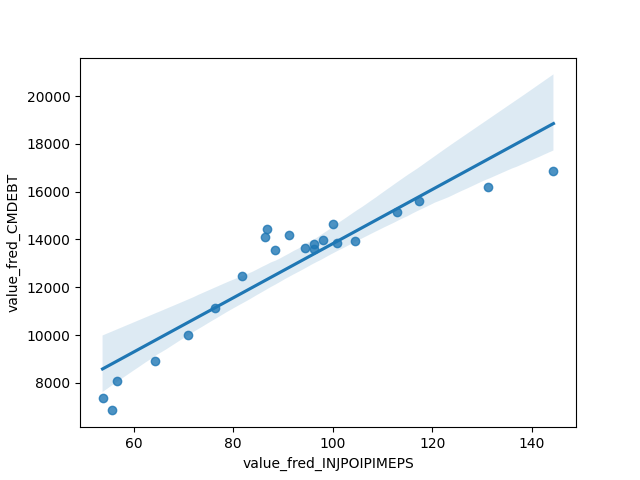
\includegraphics[scale = 0.9]{plots/plot_2025-01-10.png}
\caption{Regression Plot for 2025-01-10}
\end{figure}
\newpage

\include{tex_things/day_2025-01-11}
\section{Date: 2025-01-12}
\noindent \textbf{Series ID: W355RC1A027NBEA} 

\noindent This series is titled Depositor and insurance services: Imputed interest paid: Rest of the world and has a frequency of Annual. The units are Billions of Dollars and the seasonal adjustment is Not Seasonally Adjusted.The observation start date is 1986-01-01 and the observation end date is 2023-01-01.The popularity of this series is 1. \\ 

\noindent \textbf{Series ID: MDOTHIOH} 

\noindent This series is titled Mortgage Debt Outstanding by Type of Holder: Individuals and Other Holders (DISCONTINUED) and has a frequency of Quarterly, End of Period. The units are Millions of Dollars and the seasonal adjustment is Not Seasonally Adjusted.The observation start date is 1949-10-01 and the observation end date is 2019-07-01.The popularity of this series is 17. \\ 

\subsection{Regression Tables and Plots}
\begin{center}
\begin{tabular}{lclc}
\toprule
\textbf{Dep. Variable:}               & value\_fred\_MDOTHIOH & \textbf{  R-squared:         } &     0.877   \\
\textbf{Model:}                       &          OLS          & \textbf{  Adj. R-squared:    } &     0.873   \\
\textbf{Method:}                      &     Least Squares     & \textbf{  F-statistic:       } &     228.8   \\
\textbf{Date:}                        &    Sun, 12 Jan 2025   & \textbf{  Prob (F-statistic):} &  3.92e-16   \\
\textbf{Time:}                        &        14:57:42       & \textbf{  Log-Likelihood:    } &   -445.88   \\
\textbf{No. Observations:}            &             34        & \textbf{  AIC:               } &     895.8   \\
\textbf{Df Residuals:}                &             32        & \textbf{  BIC:               } &     898.8   \\
\textbf{Df Model:}                    &              1        & \textbf{                     } &             \\
\textbf{Covariance Type:}             &       nonrobust       & \textbf{                     } &             \\
\bottomrule
\end{tabular}
\begin{tabular}{lcccccc}
                                      & \textbf{coef} & \textbf{std err} & \textbf{t} & \textbf{P$> |$t$|$} & \textbf{[0.025} & \textbf{0.975]}  \\
\midrule
\textbf{const}                        &    4.229e+05  &     3.67e+04     &    11.508  &         0.000        &     3.48e+05    &     4.98e+05     \\
\textbf{value\_fred\_W355RC1A027NBEA} &    5.579e+04  &     3688.138     &    15.128  &         0.000        &     4.83e+04    &     6.33e+04     \\
\bottomrule
\end{tabular}
\begin{tabular}{lclc}
\textbf{Omnibus:}       &  0.965 & \textbf{  Durbin-Watson:     } &    0.575  \\
\textbf{Prob(Omnibus):} &  0.617 & \textbf{  Jarque-Bera (JB):  } &    0.995  \\
\textbf{Skew:}          &  0.334 & \textbf{  Prob(JB):          } &    0.608  \\
\textbf{Kurtosis:}      &  2.493 & \textbf{  Cond. No.          } &     17.4  \\
\bottomrule
\end{tabular}
%\caption{OLS Regression Results}
\end{center}

Notes: \newline
 [1] Standard Errors assume that the covariance matrix of the errors is correctly specified.

\begin{figure}
\centering
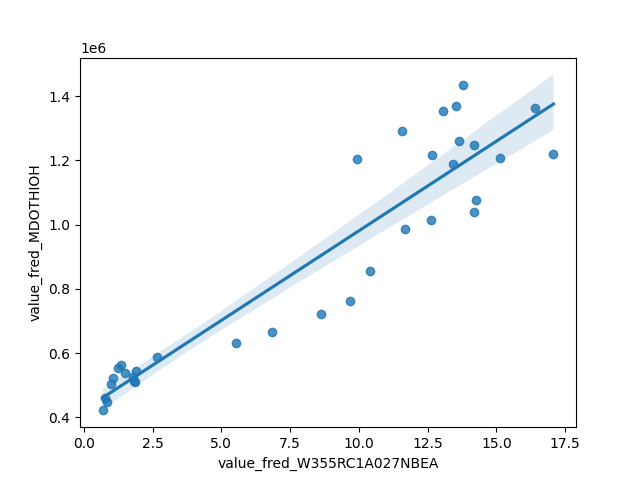
\includegraphics[scale = 0.9]{plots/plot_2025-01-12.png}
\caption{Regression Plot for 2025-01-12}
\end{figure}
\newpage


\end{document}
